%!TEX root = ../main.tex
%Adding the above line, with the name of your base .tex file (in this case "thesis.tex") will allow you to compile the whole thesis even when working inside one of the chapter tex files
%%
%%

%%%%%%%%%%%%%%%%%%%%%%%%%%%%%%%%%%%%%%%%%%%%%%%%%%%%%%%%%%%%%%%%%%%%%%%%%%%%%
%%%%%%%%%%%%%%%%%%%%%%%%%%%%%%%%%%%%%%%%%%%%%%%%%%%%%%%%%%%%%%%%%%%%%%%%%%%%%
%%%%%%%%%%%%%%%%%%%%%%%%%%%%%%%%%%%%%%%%%%%%%%%%%%%%%%%%%%%%%%%%%%%%%%%%%%%%%
%
%						RESULTS & INTERPRETATION
%
%%%%%%%%%%%%%%%%%%%%%%%%%%%%%%%%%%%%%%%%%%%%%%%%%%%%%%%%%%%%%%%%%%%%%%%%%%%%%
%%%%%%%%%%%%%%%%%%%%%%%%%%%%%%%%%%%%%%%%%%%%%%%%%%%%%%%%%%%%%%%%%%%%%%%%%%%%%
%%%%%%%%%%%%%%%%%%%%%%%%%%%%%%%%%%%%%%%%%%%%%%%%%%%%%%%%%%%%%%%%%%%%%%%%%%%%%



\onehalfspacing
\chapter{Data Analysis \& Results}
\label{chap:obs}
This chapter describes observational efforts with I-LOFAR in single station mode along with an overview of the telescope backends being used to carry out the observations. The results of initial work with TBB data and a description of analysis software are presented. An interferometric observation of a Type III radio burst and the implication of its study is described.   

\section{Observing High Temporal Resolution}
The major problem in radio astronomy currently is the computing power necessary to analyse the enormous amounts of data generated. For example, one hour of observation with I-LOFAR results in 1.3 TB of data being recorded. In order to store this stream of data from I-LOFAR, two computer clusters have been developed in the Rosse Observatory in Birr, the REALtime Transient Acquisition cluster (REALTA) and the TBB Acquisition Cluster (TACl). Both clusters are connected to I-LOFAR via 10 Gbps fibre optic cable and record data from the RSPs and TBBs respectively.
Once recorded, the challenge of analysing vast amounts of data remains. Software to display simple previews of data has been developed and efforts are underway for a more efficient solution.

\subsection{The REALtime Transient Acquisition cluster (REALTA)} 
\label{sec:REALTA}
REALTA is a 6 node computer cluster designed specifically to perform high speed de-dispersion on incoming RSP data in order to search for fast radio transients. The physical hardware has been in place since August 2018 and first light data was obtained on September 21st 2018. Despite being designed for fast radio transients, it is also of useful for observing other astrophysical phenomena with high temporal variability such as solar radio bursts and pulsars. The hardware for REALTA was purchased predominantly by University College Cork while a storage node and uninterruptable power supply were supplied by National University of Ireland, Galway. The head node is provided by the Breakthrough Listen initiative. Table \ref{table:REALTAspecs} shows the hardware specifications for the different nodes that make up REALTA.

The core computing power of REALTA comes from its 4 Dell PowerEdge R740XD servers. These each have 64 CPU cores, 256 GB of RAM and an NVIDIA Telsa V100 16 GB GPU. This makes REALTA ideal for powerful, parallel computing tasks. In its current state, data is recorded to one compute node where it is analysed afterwards however, we are currently collaborating with Griffin Foster from the Breakthrough Foundation to implement computer code that utilises REALTA's 4 powerful GPUs in order to analyse data as it is recorded. 
%The 4 PowerEdge R740XD servers perform the vast majority of all data acquisition and processing for REALTA. They can be used either individually or as part of a distributed system controlled by the headnode. Work to date has involved the RSP data link going directly to UCC1 where it is either saved directly or lightly parsed.Future plans involove moving this link to a storage node from which the data can be replicated to each of the UCC nodes.


\begin{center}
\begin{table}[ht]
\centering
\caption[Table of hardware specifications for REALTA]{Table of hardware specifications for REALTA}

\begin{tabular}{l|l|l|l}

 & Compute Node & Storage Node & Head Node \\
\hline
CPU       &  Intel Xeon Gold 6130        & Intel Xeon E5-2640      & Intel Xeon Silver 4110        \\
Clock Speed & 2.10 GHz & 2.40 GHz & 2.10 GHz \\
No. Cores & 64 & 40 & 32 \\
RAM       & 256 GB          & 256 GB        & 93 GB        \\
Storage   & 68 TB (total)          & 128 TB        & N/A        \\
GPU & 16GB NVIDIA Tesla V100 & N/A & N/A 

\end{tabular}

\label{table:REALTAspecs}
\end{table}

\end{center}



\subsection{REALTA Data Analysis}
%REALTA reads UDP packets from 4 RSP "lanes" from the I-LOFAR RSP boards. Current work has included dumping all incoming traffic from these lanes to a raw file for further processing and using capturing and parsing the data using code provided by Olaf Wucknitz.
%Data recorded with REALTA is primarily done in conjunction with a Very Long Baseline Interferometry (VLBI) pulsar observation campaign. Solar data was recorded at the time of a C5 class solar flare on January 26$^{th}$ but unfortunately no radio activity was observed.
Data is sent from I-LOFAR to REALTA using the User Datagram Protocol (UDP) along a 10 Gbps fibre optic link. The UDP data packet structure consists of a 16 byte header followed by 7808 bytes of data. Currently, data is stored on disk in this raw format and must be parsed at a later stage before analysis can be performed.

To date, some of the only data recorded with REALTA have been pulsar observations as part of a Very Long Baseline Interferometry (VLBI) pulsar observation campaign. Solar observations were made during the time of a C5 class flare on January 29th 2019. Unfortunately, this was a radio quiet event and the spectrum showed little of interest. Figure \ref{fig:blank_dspec} shows the dynamic spectrum recorded from 11:30 UTC on 2019-01-26.
\begin{figure}[t]
    \centering
    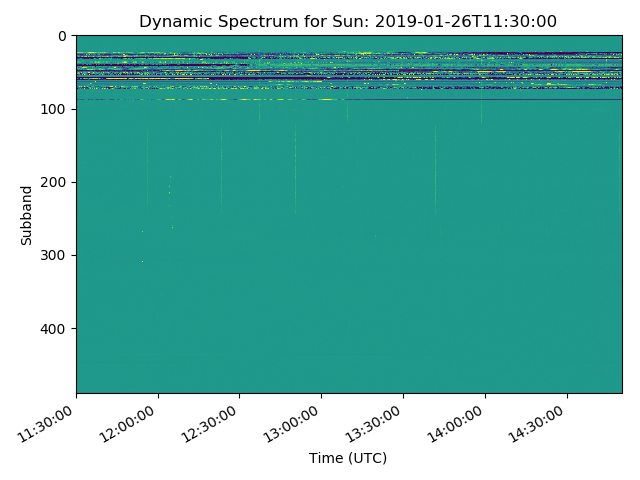
\includegraphics[width=0.5\columnwidth]{Images/Sun_dspec.png}
    \caption[Dynamic spectrum of the Sun on January 29th 2019.]{Dynamic spectrum of the Sun on January 29th 2019 from an observation made with REALTA. The time resolution here has been averaged to 8.1 ms in order to showt the full duration of the observation. A solar flare occurred at 13:21 UTC however no radio activity was detected. The intense bands below subband 100 are due to radio frequency interference (RFI) from short wave radio. Faint vertical lines can be seen between subband 122 and 244 and indicate that a number of packets have been lost between the 4 RSP lanes.}
    \label{fig:blank_dspec}
\end{figure}

\subsection{The TBB Acquisition Cluster (TACl)}
\label{sec:TACl}
TACl is a 6 node computer cluster dedicated to the recording and storage of I-LOFAR TBB data. TACl consists of 4 Dell PowerEdge SC1425 servers, an Isilon IQ 9000X storage server and an Isilon IQ 36NL storage server.
TBB data is recorded to TACl solely by the Isilon IQ 9000X storage server. This is configured in RAID6 in order to write incoming UDP packets containing TBB data to disk. This storage server has 12 disk slots, 8 of which contain Hard Disk Drives (HDDs) that write and store the incoming TBB data at $\sim$ 300MB/s. The remaining 4 slots house 2 disks containing the operating system and 2 Solid State Drives (SSDs) which are being tested as replacements for the HDDs due to their faster data writing speed. The main hurdle in recording TBB data is the disk write speed of TACl. The current solution is to delay each packet so that the previous one can be written to disk. Unfortunately, this increases the amount of time to record on full TBB dump by a great deal, something we hope to overcome by updating the HDDs to faster SSDs.

The Isilon IQ 36NL storage server is intended as general purpose for both TACl and REALTA. Currently most of this storage server is empty containing only one 1 TB HDD and 2 OS disks. Due to the fact that Ubuntu OS and mdraid do not limit storage size, the total possible storage capacity for the Isilon IQ 36NL storage server is  $34 \times 1,2,4,8,16...$TB. 

The Dell PowerEdge SC1425 servers are currently unused but are intended for light data post-processing or could possibly act as a buffer for incoming TBB data using a similar idea to LOFAR's best effort buffer.

Detailed hardware specifications of each server in TACl are shown in Table \ref{table:TAClspecs}.

\begin{center}
\begin{table}[ht]
\centering
\caption[Table of hardware specifications for TACl]{Table of hardware specifications for TACl}
\begin{tabular}{l|l|l}

 & Isilon IQ 9000X & Isilon IQ 36NL \\
\hline
CPU       &  Intel Xeon E5335        & Intel Xeon E5410            \\
CPU Clock Speed & 2.00GHz & 2.33GHz  \\
No. CPU Cores & 4 & 4  \\
RAM       & 1GB          & 4GB            \\
Storage   & 48TB          & 1TB           
\end{tabular}

\label{table:TAClspecs}
\end{table}

\end{center}

It must be acknowledged that without the tireless work of Joe McCauley neither TACl or REALTA would be in their current operational state and recording data from I-LOFAR would be limited to 1 second resolution ``beamlet statistics files".

\subsection{TBB Data Analysis}
\label{sec:tbb_data}
Data recorded using the TBBs are the real voltages induced in the antennas due to radio electromagnetic radiation. The simplicity of this data type makes it incredibly versatile and allows for a ``DIY radio telescope" approach to data analysis. This means that, because TBBs only record voltages at the antenna level they are sensitive to the entire sky. This in turn, means that beamforming can be done in any direction \textit{after} an observation has been made. Beamforming in all directions simultaneously implies imaging in all directions too but this is a much more computationally intensive task. A dedicated high performance computing cluster would be required to maximize the science output of all TBB data recorded. In its current form TACl is mostly useful for recording data only with REALTA doing the bulk of any processing work. Soon, however, REALTA will become dedicated to RSP data and the infrastructure of TACl will have to be improved.

Like RSP data, TBB data is sent from I-LOFAR using UDP packets. This is written to disk with the TBB datawriter described by \cite{Veen2015} in the form of hdf5 format files. This stores both header information and data in a standardised file format making it easily accessible.

First results from analysing TBB data and the analysis software used are described in section \ref{sec:tbb_results} along with a discussion on why further analysis of TBB data has been postponed. 

%Initial efforts in analysing TBB data are described in section \ref{sec:tbb_results} along with a discussion on the temporary discontinuation of this process.
%Initial work in this PhD was centred around obtaining the highest temporal resolution observations of the Sun to date. The task was to use I-LOFAR's TBBs to constantly monitor the Sun and to output when something of interest occurred. Unfortunately, this task requires a lot of technical knowledge and an adequate computer and network set-up, neither of which were present. Regardless, software to beamform data from TBBs was developed and a TBB correlator was utilised to produce prototype dynamic spectra and all-sky images.

%\subsection{Motivation for Study}%(This is why they matter/ what you should have learned)}
%Type III radio bursts are a prevalent feature of radio emission from the Sun. They can occur individually or occasionally in the form of Type III storms which consist of continuous Type III bursts that can last up to days. The defining characteristic of Type III bursts can be recognised in dynamic spectra as a rapid frequency drift from high to low frequencies (see Figure \ref{fig:bursts}). In the case of Type IIIb bursts there exists a fragmented substructure. Other variations of Type III bursts include reverse or bidirectional bursts, which have a positive frequency drift, and U and J bursts, which both show a turning point in frequency drift.

%Type III bursts are caused by electron beams travelling through a slower background of plasma leading to a bump-on-tail instability in the plasma. This means that a positive gradient in the velocity distribution is formed, leading to an instability that causes a rapid growth in the magnitude of Langmuir waves (see Eq. \ref{eq:dWdt}. These Langmuir waves then undergo decay or coalesce with ion sound waves or backward propagating Langmuir waves to produce radio emission at the plasma frequency and its second harmonic respectively. The instability in Langmuir waves is resolved by a diffusive term in Eq. \ref{eq:dfdt} that broadens the bump-on-tail to a plateau, eliminating the positive gradient.

%The study of radio emission from the Sun, Type III bursts in particular, is just as active now as it was immediately after WW2. New instruments like LOFAR and MWA are being used in various ways to observe and study Type III bursts and their sub-categories \citep{Morosan2014,Reid2017ImagingLOFAR, McCauley2017}. The study of Type III bursts give us an insight into the magnetic reconnection that takes place during solar flares. This has implications in space weather research which can have widespread effects here on Earth.

%With new discoveries being made on a regular basis, long disputed questions are being answered and new questions are being asked. The development of the next generation of radio interferometers, the Square Kilometre Array (SKA), will hopefully bring about a new world of information on Type III bursts and the plasma processes that generate them.
%\subsection{Solar Transient Features}
%One of the goals of this PhD is to use REALTA and TACl to observe a number of solar transient features at the highest resolution to date. Current progress on TACl has been slow due to technical problems in TBB data capture and REALTA is operational in a minimal sense however, both show enormous potential for the future. Recent publications on Sbursts, TypeIIIbs and many more show that there is much to be learned if we just had the resolution!

\section{Observing High Spatial Resolution}
\label{sec:event}
The second aspect of this PhD is to study high spatial resolution observations of a solar radio burst. One of the fundamental questions about solar radio observations is: are source sizes what they are observed to be or does scattering in the corona have a major effect? Interferometric observations from LOFAR are one of the best methods of testing this hypothesis, especially if the remote and international stations can be used to generate the longest baselines resulting in sub-arcminute and even sub-arcsecond resolution.

In order to learn more about fine structural scale in the corona and the degree to which scattering affects radio emission, an interferometric dataset of a Type III radio burst is being analysed. The data is taken from 2015-10-17 using all of the core LOFAR stations and 12 of the remote stations, a total of 36 stations, yielding 630 baselines with a maximum of 84 km.
The Type III burst which occurred at 13:21 UTC is briefly described in appendix \ref{app:event}. A spectrum of the Sun was recorded using the LOFAR remote station RS509 from 2015-10-17 08:00 UTC to 2015-10-17 14:00 UTC. The Type III burst is observed in this spectrum at approximately 13:21 UTC as shown in Figure \ref{fig:LOFAR_spec}. Figure \ref{fig:LOFAR_spec} shows the variability in emission of the burst. It is immediately obvious that the Type III burst shows striations, the implications of this will be discussed below.
\begin{figure}
    \centering
    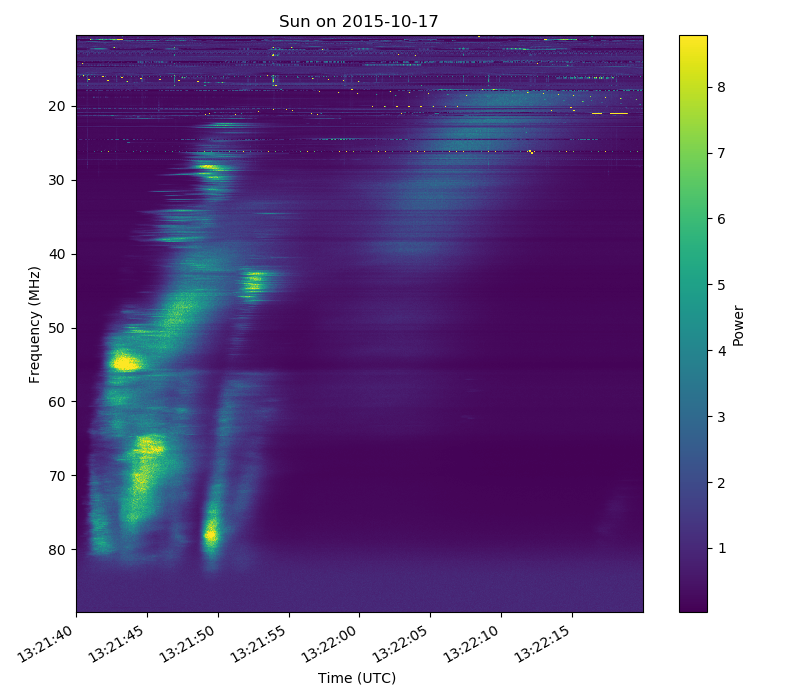
\includegraphics[width=0.75\columnwidth]{Images/L401005_SAP000_B000_S0_P000_bf_d_spec_burst_zoom.png}
    \caption[Type III radio burst observed with LOFAR station RS509]{a) Type III radio burst observed with LOFAR station RS509 in the north of the Netherlands. A plethora of temporal and frequency variation can be seen over the burst's duration.}
    \label{fig:LOFAR_spec}
\end{figure}
% The Type III burst which occurred at 13:21 UTC is shown in the composite radio spectra in Figure \ref{fig:comp_spec} and was not co-temporal with any other solar event.

% \begin{figure}
%     \centering
%     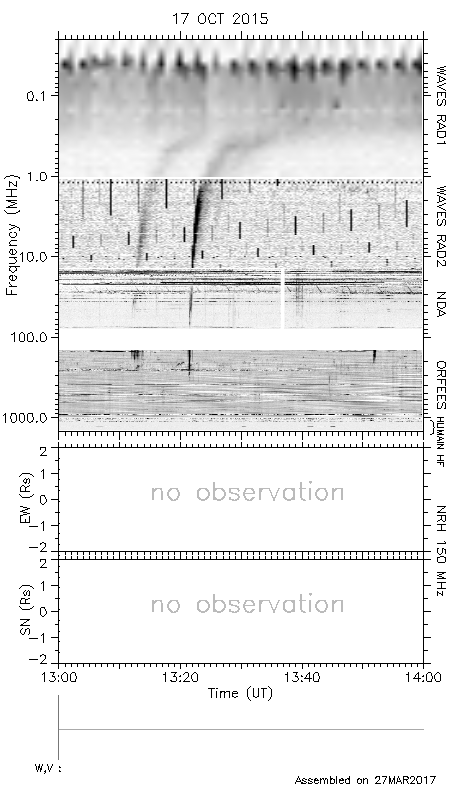
\includegraphics[width=0.75\columnwidth]{Images/Radio_composite.png}
%     \caption[Composite of radio spectra from multiple ground and space based radio telescopes.]{Composite of radio spectra from multiple ground and space based radio telescopes. From top to bottom these include; WAVES RAD1, WAVES RAD2 (both on board the WIND space craft), the Nan\c{c}ay Decametric Array (NDA), ORFEES radio-spectrograph (Observations Radio pour Fedome et l’Etude des Eruptions Solaires) and the Nan\c{c}ay Radio Heliograph (NRH, no data). A Type III radio burst is seen as a dark streak after 13:20 in all 4 spectra.}
%     \label{fig:comp_spec}
% \end{figure}

% EUV images of the Sun such as those taken in the 193{\AA} channel with AIA, Figure \ref{fig:AIA_GOES}a, show a number of bright active regions and a coronal hole which give indications of where to expect closed and open magnetic field lines.
% Xray flux around the time of the Type III burst was measured by the Geostationary Operational Environmental Satellite (GOES, seen in Figure \ref{fig:AIA_GOES}b). It should be noted that there were a number of small C class solar flares before the radio burst however none were co-temporal. 


% \begin{figure}
%     \centering
%     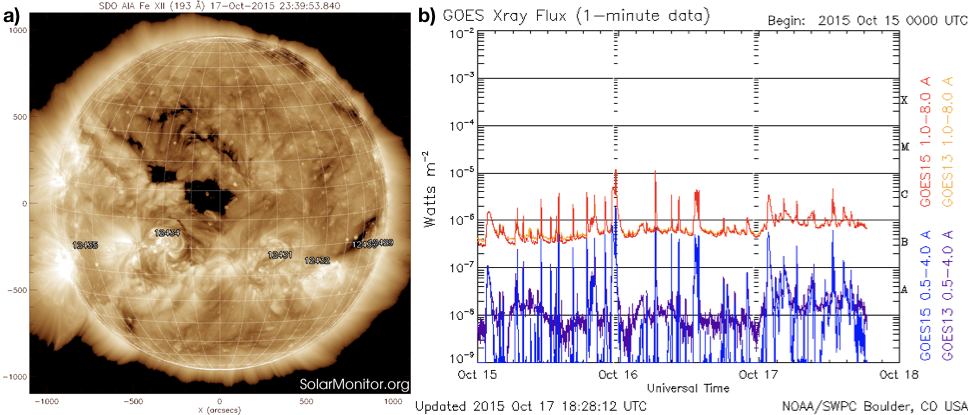
\includegraphics[width=\columnwidth]{Images/aia_goes.png}
%     \caption[193 {\AA} image of the Sun taken by AIA and Xray flux as measured by GOES on 2015-10-17]{a) 193 {\AA} image of the Sun taken by AIA on 2015-10-17 b) Xray flux as measured by GOES on 2015-10-17.}
%     \label{fig:AIA_GOES}
% \end{figure}


% % \begin{figure}
% %     \centering
% %     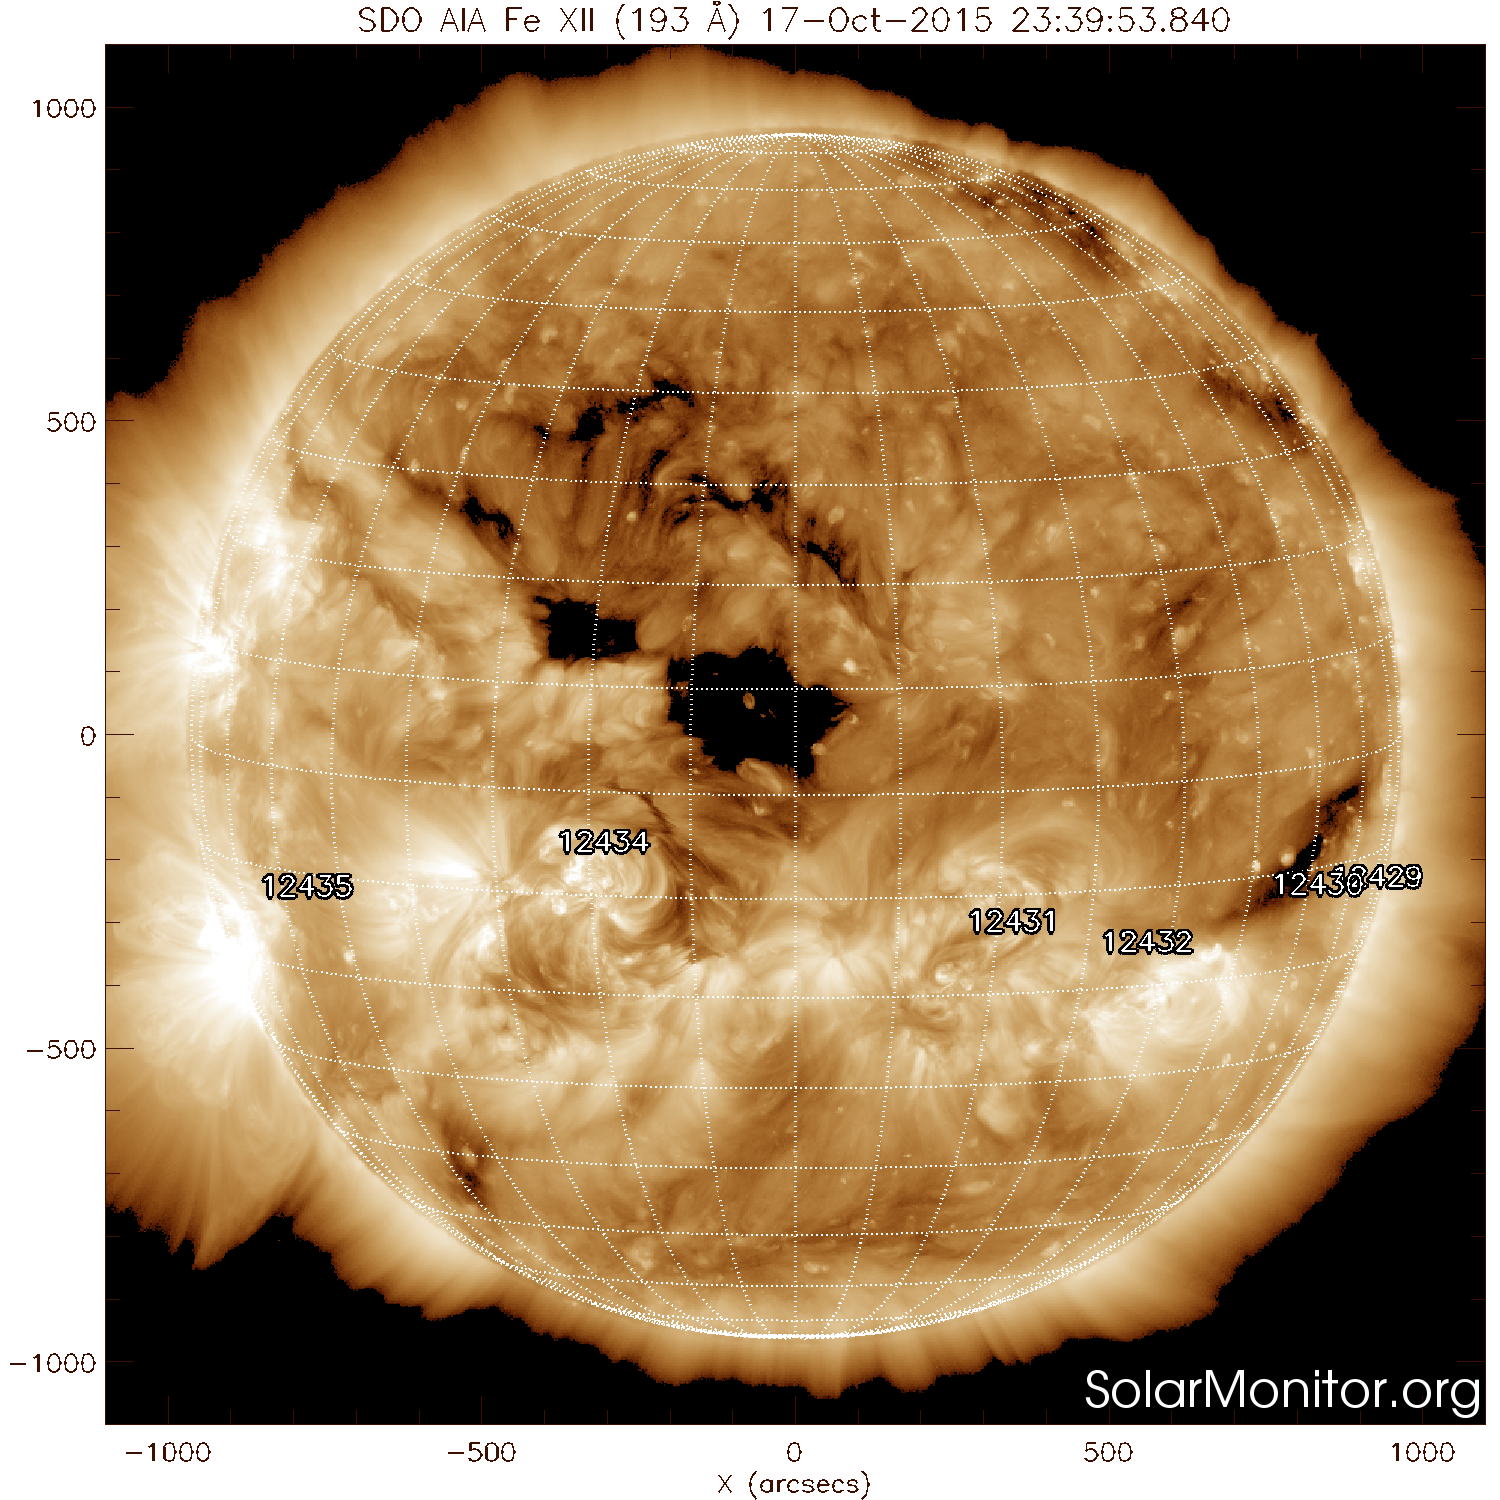
\includegraphics[width=0.75\columnwidth]{Images/aia_193.png}
% %     \caption[193 {\AA} image of the Sun taken by AIA on 2015-10-17]{193 {\AA} image of the Sun taken by AIA on 2015-10-17}
% %     \label{fig:aia193}
% % \end{figure}

% A spectrum of the Sun was recorded using the LOFAR remote station RS509 from 2015-10-17 08:00 UTC to 2015-10-17 14:00 UTC. The Type III burst is observed in this spectrum approximately 19300s after the observation start as shown in Figure \ref{fig:LOFAR_spec}a. Figure \ref{fig:LOFAR_spec}b shows the burst over a shorter time scale thus allowing the variability in emission to be seen.
% \begin{figure}
%     \centering
%     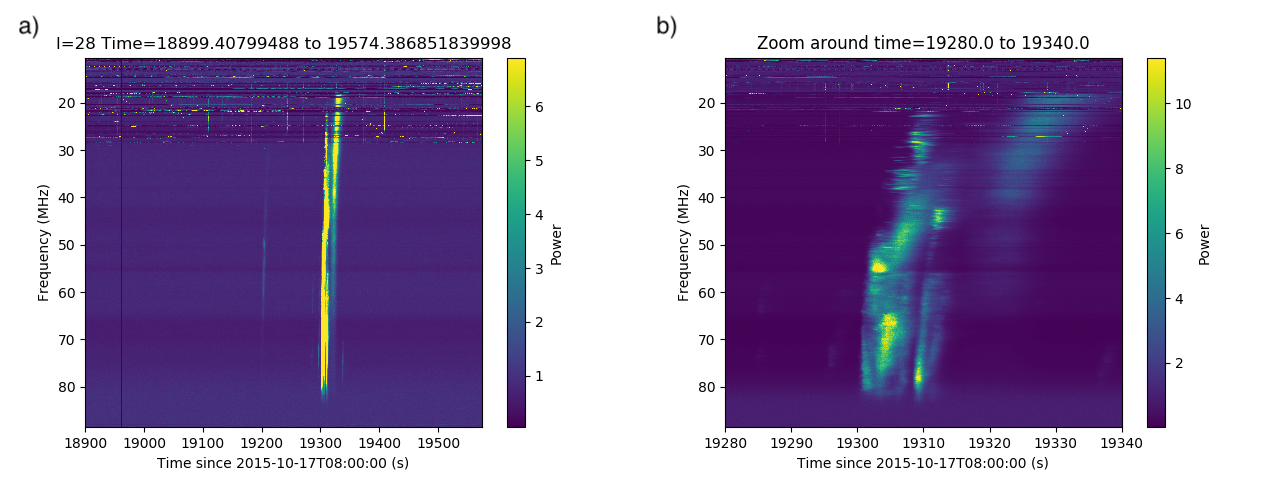
\includegraphics[width=\columnwidth]{Images/L401005_SAP000_B000_S0_P000_bf_d_spec_composite.png}
%     \caption[Type III radio burst observed with LOFAR station RS509]{a) Type III radio burst observed with LOFAR station RS509 in the north of the Netherlands. b) A zoom in of the Type III burst, a  plethora of temporal and frequency variation can be seen over the burst's duration.}
%     \label{fig:LOFAR_spec}
% \end{figure}

The most common observational method for Type III bursts with LOFAR is the tied-array imaging mode \citep{Morosan2014} whereby a number of LOFAR ``station beams", formed by combining all the antennas in a single LOFAR station, are added coherently to create tied-array beams. These beams are then tessellated across the Sun and an image reconstructed from the spectra of each beam. This imaging mode has the benefit that it retains the 5.12 $\mu$s resolution but accurately determining source size and position becomes an issue due to multiple beams detecting radio emission. Interferometric imaging therefore gives a more accurate spatial resolution of a burst at the cost of one image every 0.25 s.


%\chapter{Results \& Interpretation}
%\label{chap:results}
%Results from TBB observations are described here along with preliminary images of a Type III burst. 

\section{TBB Results}
\label{sec:tbb_results}
The initial work during this PhD was done on building a data analysis pipeline for TBB data from I-LOFAR. At the time, TACl (section \ref{sec:TACl}) was still in its early stages of operation and testing of data acquisition method indicated much more needed to be done to capture TBB data at a sufficient rate. Despite this, a moderate codebase (\url{https://github.com/ILOFAR/TBB_scripts}, described below) was created in order to analyse this ``commissioning data". This software allows TBB data to be beamformed in any direction on the sky to produce a dynamic spectrum such as the prototype dynamic spectrum of the Sun in Figure \ref{fig:proto_dspec}. These dynamic spectra can cover any frequency range within the observed band with the limiting factor on frequency resolution being computer power and the size of the Fourier window. Section \ref{sec:TBB_software} describes how the software written in the first few months of this PhD produced the highest temporal resolution observations ever achieved.
\begin{figure}
    \centering
    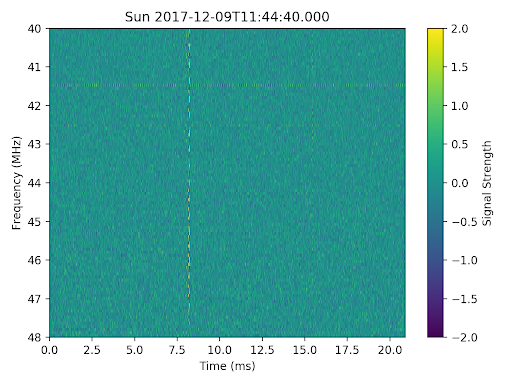
\includegraphics[width=0.5\columnwidth]{Images/TBB_dspec.png}
    \caption[Prototype TBB dynamic spectrum]{A prototype TBB dynamic spectrum created using code written in the first few months of this PhD.}
    \label{fig:proto_dspec}
\end{figure}


A correlator for TBB data (\url{https://github.com/sabourke/tbb-correlator}) was utilised to produce the prototype all sky image of Figure \ref{fig:proto_allsky}a. In order to correlate data correctly, all input data must have the exact same start time. This criterion was only fulfilled by 7 antennas leading to poor a \textit{uv} coverage. Figure \ref{fig:proto_allsky}b shows the point spread function (PSF) of the 7 element array which is shown to have several bright spots in a pattern around the main beam, these are the sidelobes of the antenna beam.
\begin{figure}
    \centering
    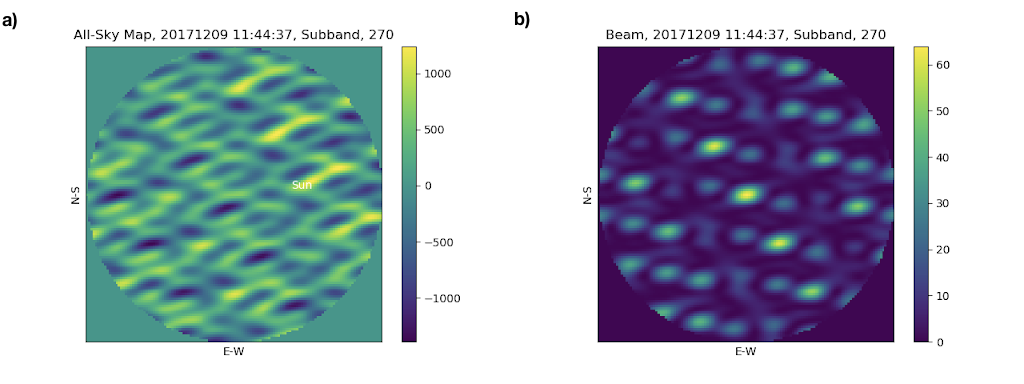
\includegraphics[width=\columnwidth]{Images/AllSky_psf.png}
    \caption[Prototype TBB all sky image]{a) A prototype all sky image made from TBB data. Technical difficulties in recording data with a precise start time meant that only data from 7 antennae could be correlated to produce this image. This resulted in the point spread function b) containing numerous sidelobes. }
    \label{fig:proto_allsky}
\end{figure}

Despite the potential of TBB data to revolutionise solar observations, difficulties in acquiring it reliably mean that development of this code and analysis of TBB data are to be postponed until analysis of an interferometric observation of a Type III burst (section \ref{sec:event}) is complete.
% beam with numerous sidelobes, this in turn produced the low quality image shown.
\subsection{TBB Software}
\label{sec:TBB_software}
In order to create dynamic spectra from TBB data, the channelisation of a LOFAR RSP board must be replicated. For brevity's sake, the following discussion will ignore the procedure to beamform as it is simply an implementation of the theory described in section \ref{sec:beamform_theory}. 

In order to preserve the 5 ns time resolution of TBB data the raw voltage data must first undergo a Fourier transform. This can be though of as representing the entire signal time series as power per frequency with frequency resolution governed by the relation from a discrete Fourier transform (DFT),
$$\Delta f = \frac{1}{N\Delta t}$$
where $\Delta f$ is the frequency resolution, $N$ is the number of points the DFT uses and $\Delta t$ is the time resolution. Depending on the desired frequency resolution, the data spectrum obtained from the DFT is then split into a number of ``subbands" which are analogous to subbands produced in an RSP board (Figure \ref{fig:subbands_pspec}a). One subband is selected while the rest of the spectrum is set to zero so that an inverse DFT can be performed resulting in the initial 5 ns time resolution. This is done for each subband so that a number of time series at a particular frequency range are created. These time series are then stacked and represented as a dynamic spectrum such as the one in Figure \ref{fig:subbands_pspec}b.

\begin{figure}
    \centering
    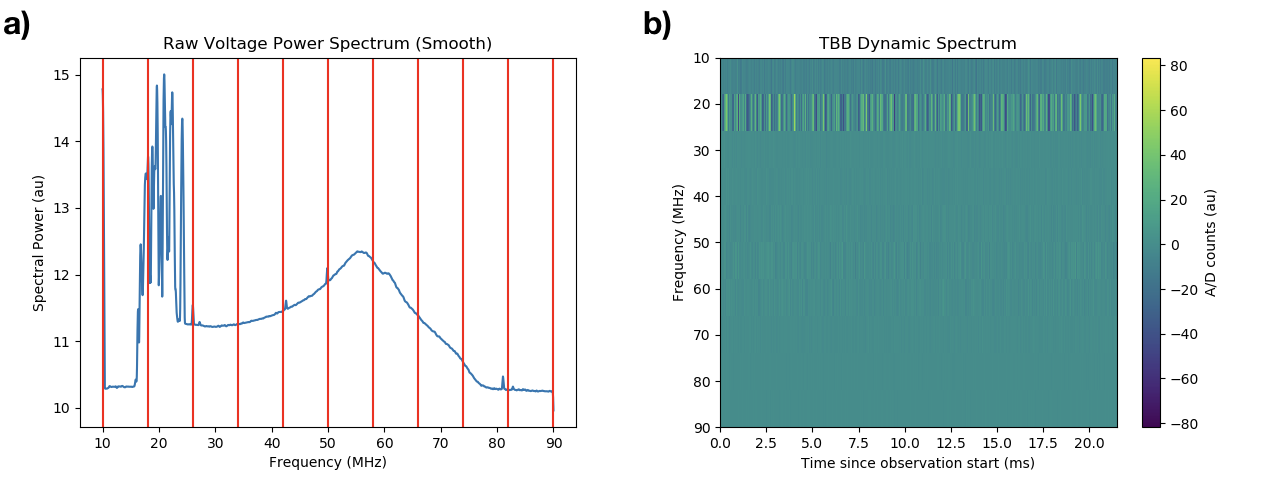
\includegraphics[width=\columnwidth]{Images/TBB_spectra.png}
    \caption[Spectrum of TBB data and subbands]{a) A sample spectrum of TBB data. The spectrum is smoothed for clarity and the subband edges are shown as red vertical lines. b) The dynamic spectrum by channelising in the method outlined above.}
    \label{fig:subbands_pspec}
\end{figure}

% \begin{figure}[t]
%     \centering
%     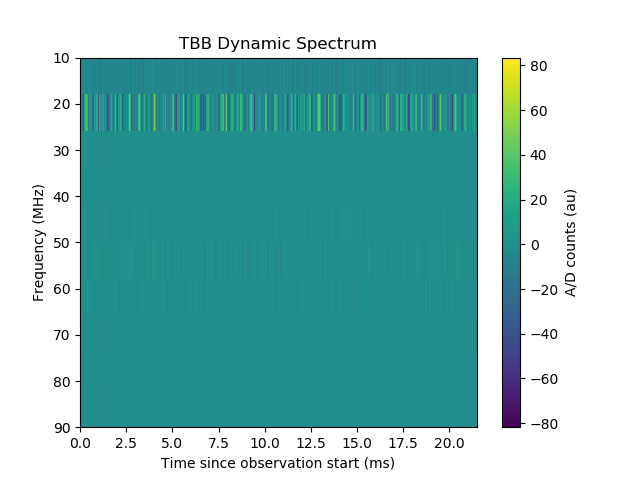
\includegraphics[width=0.75\columnwidth]{Images/TBB_dynamic_spectrum.png}
%     \caption[Dynamic spectrum of TBB data]{The dynamic spectrum by channelising in the method outlined above.}
%     \label{fig:TBB_dspec}
% \end{figure}

Performing channelisation in this way gives a user the freedom to select any frequency range to channelise within the band with any frequency resolution. There are however, a few undesired effects of too fine a frequency resolution. Firstly, windowing a DFT produces unwanted sidelobes in the reconstructed time series and also serves to broaden sharp peaks. Before further work can be done using this code, the effects of different DFT window sizes must be characterised.

Once TACl can record TBB data reliably, development and implementation of the existing code can continue. It is hoped that by the end of this PhD that ``quick look" plots of TBB data can be produced in almost real time as the data is being recorded in order to automatically discern whether there is an event of interest or if the data can be deleted. It is expected that a number of machine learning algorithms will be utilised in this process.

\section{Interferometric Results}
Figure \ref{fig:typeIIIcomp} shows a number of preliminary interferometric images at different wavelengths of the Type III burst described in appendix \ref{app:event}. Here, 4 subbands corresponding to 29.68 MHz, 39.45 MHz, 49.21 MHz and 63.28 MHz of the burst are displayed at the time 13:21:55.6. The red crosses in each panel indicate the centre of the Sun and the point of maximum intensity in the burst, the red circle shows the size of the Sun.
This type of interferometric observation gives a great opportunity to study Type III emission from the perspective of both burst dynamics and radio wave propagation. Positional tracking of a Type III burst was carried out by \cite{Mann2018} and is the only study of its kind. However, the dynamic spectra were reconstructed from the images and not recorded in LOFAR beam-formed mode, as is the case for this observation. % Thus, more detailed spectral and temporal characteristics than the be studied.
Type III bursts are sometimes observed to contain fine spectral structures known as striae. These can be used to give an order of magnitude limit to the source size of density inhomogoneities in the solar corona as was described in \cite{Kontar2017}. 
The Type III burst captured in this data also contains striae (Figure \ref{fig:LOFAR_spec}) meaning a direct comparison with \cite{Kontar2017} can be made. Controversy exists as to whether the conclusions from \cite{Kontar2017} are a result of coronal scattering, as claimed, or are due to the extended beam size of tied-array imaging. Analysis of the event described above will be a further piece of evidence in support of/against the importance of coronal scattering.

%thus clearing some controversy in the solar community as it will be the first time this study is done using interferometric imaging instead of tied-array imaging.

From the preliminary images in Figure \ref{fig:typeIIIcomp} it is immediately obvious that the source sizes in these images are smaller by a large amount than suggested by \cite{Kontar2017} who present source sizes of the order 20 arcminutes. %The Type III source can be seen at a greater distance from the Sun with decreasing frequency as expected from the plasma emission theory of Type III bursts, which suggests that lower frequencies correspond to lower electron densities and thus, greater heights in the solar corona.
\begin{figure}[t]
    \centering
    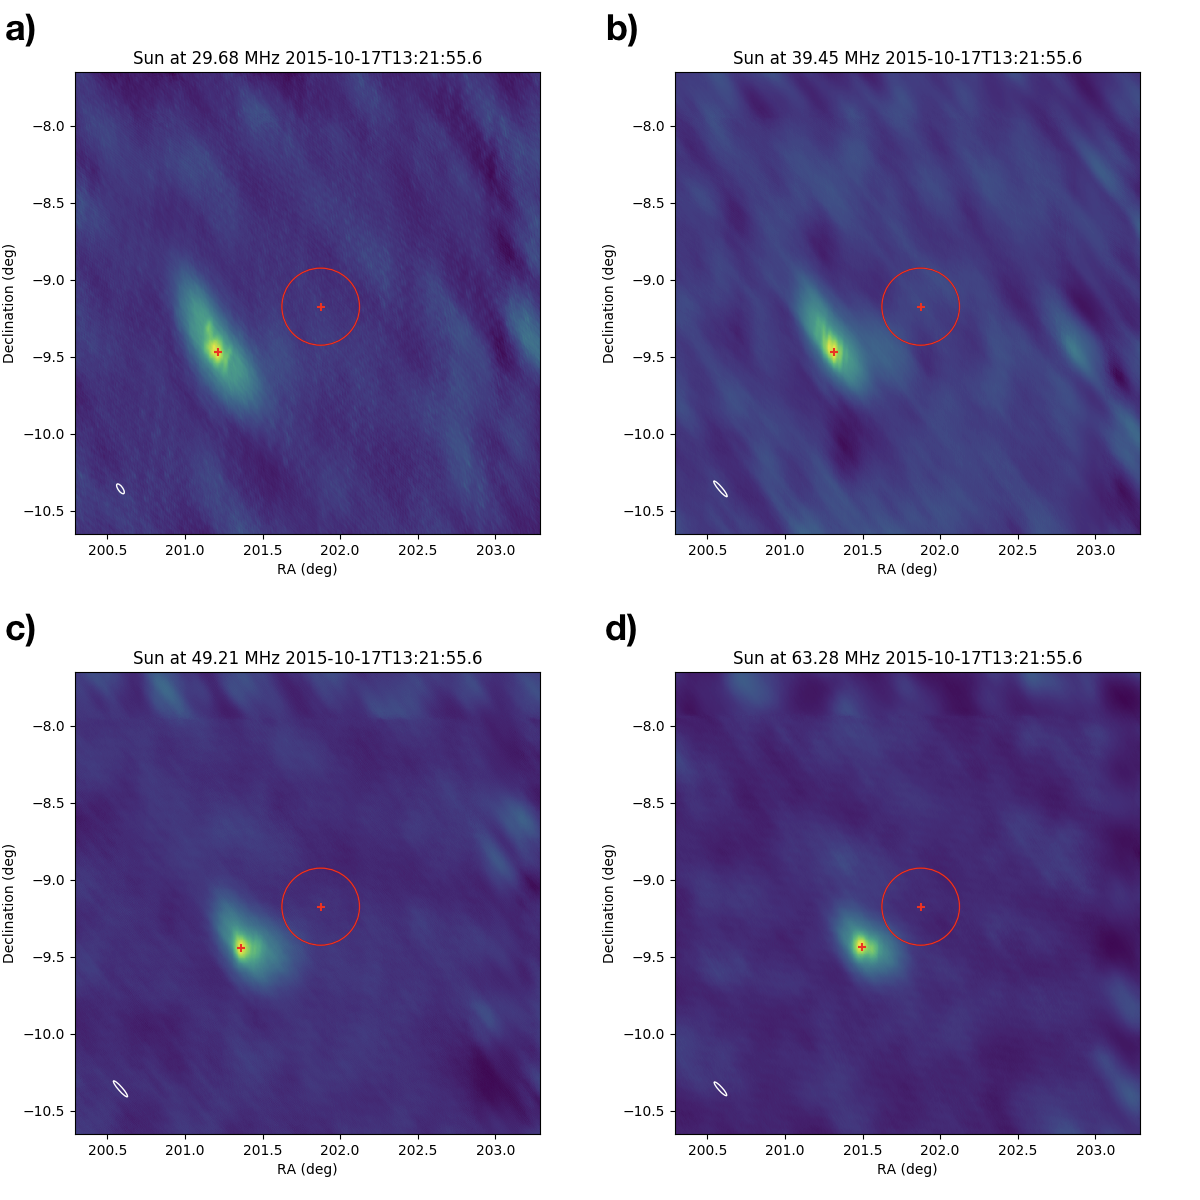
\includegraphics[width=0.75\columnwidth]{Images/TypeIII_comparison.png}
    \caption[Interferometric images of a Type III burst]{Interferometric images of a Type III burst at 13:21:55.6 on 2015-10-17 at 4 different frequencies a) 29.68 MHz b) 39.45 MHz c) 49.21 MHz d) 63.28 MHz. The red circle in each panel indicates the size of the Sun and the two red crosses indicate the centre position of the Sun and the position of maximum intensity in each panel. The with ellipse indicates the shape and position of the LOFAR beam.}
    \label{fig:typeIIIcomp}
\end{figure}

The images I have created thus far have yet to undergo a thorough analysis of the effects of parameters used in the WSCLEAN algorithm \citep{Offringa2014}, one of the main deconvolutional methods used to produce interferometric images. Different weighting schemes prioritise different spatial scales in interferometric observations. Knowing that coronal scattering may effect observed source sizes, extreme care must be taken before any conclusive inferences are drawn from images produced. An initial inspection of Figure \ref{fig:typeIIIcomp} suggests the source size of the Type III burst to be of the order of the size of 0.5 R$_{\odot}$ at lower frequencies and $\sim 1 \mbox{ R}_\odot$ at higher frequencies. 










